% CLASE
\documentclass[a4paper,12pt]{article}

% PREÁMBULO
% Paquetes:
\usepackage[spanish]{babel}
\usepackage{graphicx}
\usepackage{tikz,color}
\usepackage{pgf-pie}
\usepackage{pgfgantt}
\usepackage{pdflscape}
\usepackage[backend=biber]{biblatex}
\usepackage[table]{xcolor}
\usepackage{multirow}
\usepackage{adjustbox}
\bibliography{Recursos/Bibliografia}

% CUERPO
\begin{document}

% Caratula
    \begin{titlepage}
        \centering
        
\includegraphics[width=0.2\textwidth]{Imagenes/LogoUTN.png}\par
        \vfill
        {\bfseries\LARGE Universidad Tecnológica Nacional \par}
        \vfill
        {\scshape\Large Facultad Regional Rosario \par}
        \vfill
        {\scshape\Huge Aplicación de Apoyo al Cuidado de Personas \par}
        \vfill
        {\itshape\Large Ingeniería en Sistemas de Información \par}
        {\itshape\Large Proyecto Final de Carrera \par}
        \vfill
        {\Large Autores: \par}
        {\Large Carignani, Esteban Agustín \par}
        {\Large Culich, María Agustina \par}
        {\Large Montisori, Agustín \par}
        \vfill
        {\Large Tutor: \par}
        {\Large Stortoni, Silvia \par}
        \vfill
        {\Large Abril 2024 \par}
    \end{titlepage}

% Abstract
    \begin{abstract}
        Cuidar de otra persona, ya sea un adulto mayor, 
        un niño, una persona con discapacidad o alguien 
        con una enfermedad, puede ser una tarea compleja. 
        La gestión de medicamentos, horarios, cuidadores, 
        turnos, recordatorios médicos y la comunicación 
        entre las personas involucradas.
        Basándonos en las respuestas de una encuesta realizada enfocada a personas que tienen a su cargo el cuidado de otras, presentamos una aplicación móvil innovadora que facilita la gestión y organización de las tareas que implica estar al cuidado de alguien más. Nuestra propuesta es una app que permitiría el registro de información personal de la persona bajo cuidado y la asociación de esta al cuidador, centralización de la comunicación entre ambas partes y terceros involucrados, simplicidad en la organización de visitas y turnos médicos, agenda de medicación, tareas cotidianas, etc. Además, se incluirán herramientas que respondan a las necesidades relevadas en el cuestionario de sondeo.
    \end{abstract}

    \newpage

% Tabla de contenidos
    \tableofcontents 
    
    \newpage

% Análisis de la organización
    \section{Analisis de la organización}
    \par Partiendo de la base en que para el proyecto no existe una organización u empresa definida particular en la cuál apoyarnos, el análisis organizacional que llevaremos a cabo pone foco principal en el equipo de desarrollo del proyecto en cuestión, considerando al mismo como una \textit{startup} que se inicia en el mercado de desarrollo de soluciones informáticas. Concentrando los esfuerzos principalmente en las capacidades y recursos del equipo a cargo.
    \par El objetivo es evaluar la estructura del equipo, habilidades, procesos de trabajo, disponibilidad de recursos financieros y tecnológicos, definición de fortalezas, debilidades y oportunidades que pueden afectar al desarrollo del equipo como organización.
    \subsection{BubiSoft}
    \par La empresa toma como punto de partida inicial el desarrollo de soluciones informáticas orientadas a problemáticas sociales y cotidianas de las personas.
    \par El mercado al que apunta la organización y sobre el cual sienta las bases de su crecimiento es el siguiente:
    \begin{itemize}
        \item Sujetos que se enfrentan ante una situación específica que deriva en la necesidad de tener una o más personas encargadas.
        \item Familiares o red de contención que se encargan del cuidado de una o más personas dependientes o parcialmente dependientes y de todas las tareas que engloba.
    \end{itemize}
    \par Tomando esto en consideración, procedemos a la realización del análisis que nos permite determinar la misión, visión y objetivos de la organización.
    \subsection{Misión}
    \par Brindar soluciones tecnológicas que simplifiquen la atención a las problemáticas cotidianas para aquellas personas que se encuentren en situación de vulnerabilidad y sirvan de apoyo para con los responsables del cuidado.
    \subsection{Visión}
    \par Posicionarse como una de las principales consultoras tecnológicas responsables de brindar soluciones informáticas innovadoras para abordar diversas problemáticas sociales.
    \subsection{Objetivos principales}
    \begin{itemize}
        \item Brindar soluciones tecnológicas que mejoren la calidad de vida de las personas mayores y faciliten la labor de sus cuidadores.
        \item Alcanzar la sostenibilidad financiera y un crecimiento rentable a largo plazo, posicionándose de forma estratégica en el mercado de soluciones informáticas.
        \item Contribuir a mejorar el bienestar general de la sociedad, estudiando y evaluando con atención sus necesidades y contribuyendo con formas de satisfacerlas a través del desarrollo de nuevas tecnologías.
    \end{itemize}
    \subsection{Objetivos secundarios}
    \begin{enumerate}
        \item \underline{Organizacionales}
        \begin{itemize}
            \item Identificar las necesidades específicas de las personas.
            \item Desarrollar soluciones tecnológicas fáciles de usar e intuitivas para los usuarios.
            \item Ofrecer funcionalidades que aborden las necesidades más comunes.
            \item Desarrollar un sólido modelo de negocio que genere ingresos a través de suscripciones.
            \item Atraer y retener usuarios.
            \item Explorar oportunidades de expansión en mercados similares.
        \end{itemize}
        \item \underline{Sociales}
        \begin{itemize}
            \item Reducir la carga de trabajo de los cuidadores y familiares.
            \item Promover la independencia y autonomía de las personas mayores.
            \item Reducir los niveles de aislamiento social y soledad de las personas mayores.
            \item Concientizar a la sociedad sobre los desafíos que representan la etapa de envejecimiento.            
        \end{itemize}
    \end{enumerate}
    \subsection{Organigrama}
    \par Si bien la empresa resulta ser una startup inicial que consta de pocas personas integrándola, realizamos el organigrama basándonos en los roles y funciones que cumplen sus integrantes.
    \par 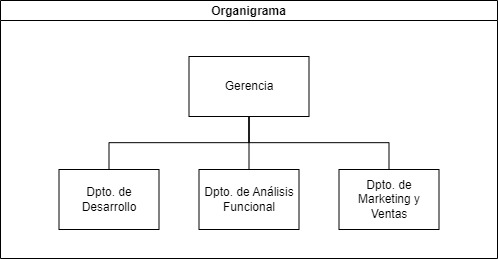
\includegraphics[width=1\textwidth]{Imagenes/Organigrama.jpg}
    \par Profundizaremos un poco más en las tareas a cargo de cada uno de los departamentos que integran a la empresa.
    \begin{itemize}
        \item[\textbf{Gerencia:}] Se compone del equipo fundador de la empresa, encargados de la toma de decisiones relacionadas al futuro de la empresa, el camino a seguir y los proyectos a encarar.
        \item[\textbf{Desarrollo:}] Es el departamento a cargo del arquitecto de software, quien coordina a todos los desarrolladores a lo largo de la codificación, desarrollo y mantenimiento del software.
        \item[\textbf{Análisis:}] Este departamento está a cargo del líder de proyectos, a su mando están los analistas y testers, encargados de relevar, comprender e interpretar las necesidades de los clientes y asegurar que las mismas se satisfagan correctamente por el software implementado.
        \item[\textbf{Marketing:}] El departamento de marketing se encarga de publicitar, publicar y promover el uso de la aplicación desarrollada. A su vez, sus tareas incliuyen realizar campañas de retención de usuarios, escuchando las críticas que estos ofrezcan, y comunicándolas al departamento de análisis. 
    \end{itemize}
    \subsection{Matriz FODA}
    \textbf{\underline{Fortalezas}}
    \begin{itemize}
        \item[] \textit{Enfoque en problemática social:} Al centrarse en atender una necesidad real y creciente de la sociedad, la empresa da un propósito claro, apuntado a un mercado real de potenciales clientes.
        \item[] \textit{Soluciones innovadoras:} La empresa propone soluciones tecnológicas novedosas y adaptadas a las necesidades específicas de las personas.
        \item[] \textit{Potencial de impacto:} Las soluciones tienen el potencial de mejorar significativamente la calidad de vida de las personas, generando un impacto positivo en la sociedad.
        \item[] \textit{Alta motivación:} Al ser una empresa que está en sus inicios, sus integrantes están altamente motivados para enfrentar los diferentes desafíos de forma proactiva e inmediata.
    \end{itemize}
    \textbf{\underline{Oportunidades}}
    \begin{itemize}
        \item[] \textit{Innovación:} Los nuevos avances en tecnología como la inteligencia artificial y la domótica pueden abrir nuevas posibilidades para el desarrollo de soluciones innovadoras.
        \item[] \textit{Creciente mercado:} De la mano con la revolución tecnológica y el amplio rango de edad que abarcan actualmente las tecnologías, genera una demanda cada vez mayor de soluciones que puedan hacer frente a las necesidades de las personas.
        \item[] \textit{Alianzas estratégicas:} La organización es capaz de asociarse con otras empresas, organizaciones o instituciones enfocadas en temáticas inherentes a las soluciones brindadas, para ampliar su alcance y potenciar su impacto.
    \end{itemize}
    \textbf{\underline{Debilidades}}
    \begin{itemize}
        \item[] \textit{Inexperiencia:} Al ser una startup reciente que incursiona en el desarrollo de soluciones tecnológicas, se enfrenta a los problemas de falta de experiencia a la hora de afrontar desafíos técnicos, financieros y de gestión.
        \item[] \textit{Capital limitado:} Cada decisión a tomar implica un potencial riesgo en la continuidad y estabilidad de la empresa debido al poco capital inicial con el que cuentan.
        \item[] \textit{Escasez de recursos:} El escaso nivel de personal inicial representa una limitante a la hora de tomar posibles proyectos debido al riesgo de caer en una sobrecarga laboral que afecte a las entregas y el éxito de los mismos.
    \end{itemize}
    \newpage
    \textbf{\underline{Amenazas}}
    \begin{itemize}
        \item[] \textit{Avances tecnológicos:} La aparición de nuevas tecnologías pueden crear soluciones a las mismas problemáticas de los proyectos realizados por la empresa pudiendo dejarlos obsoletos.
        \item[] \textit{Dificultades para obtener financiación:} sin el apoyo de programas gubernamentales y organizaciones sin fines de lucro, podría limitar la capacidad de la organización para crear nuevas soluciones.
        \item[] \textit{Mercado competitivo:} El gran nivel de demanda y competencia salarial que presenta el actual mercado de tecnología, dificulta el ingreso competitivo y la rentabilidad inmediata de la empresa.
    \end{itemize}
    \subsection{Procesos principales}
    \par Tomando en consideración el análisis hecho de la organización, y el foco que hacen en las problemáticas sociales, consideramos los siguientes procesos principales.
    \newline
    \par \noindent \textbf{\underline{Investigación y desarrollo}} \newline
    \par Dentro de los procesos de investigación y desarrollo incluimos procesos más atómicos cómo:
    \begin{itemize}
        \item[] \textit{Identificación de necesidades:} este proceso engloba la realización de un análisis de las necesidades específicas de los stakeholders tanto a nivel individual cómo a nivel colectivo. Dentro del mismo se engloban tareas cómo la realización de encuestas, entrevistas, grupos focales, etc., que permitan comprender los desafíos y oportunidades que enfrentan.
        \item[] \textit{Diseño y modelado de soluciones:} consiste en diseñar las posibles soluciones tecnológicas innovadoras que hagan frente a las necesidades identificadas previamente, priorizando la facilidad de uso y las capacidades de los usuarios a los que apunta. Se emplean metodologías de modelado centradas en la experiencia de usuario para asegurar la conformidad y usabilidad de las aplicaciones.
        \item[] \textit{Desarrollo de software:} este proceso engloba todas las tareas relacionadas a la materialización de las propuestas tecnológicas planteadas y diseñadas previamente. Se definen y emplean metodologías de desarrollo acordes a las necesidades de cada proyecto y herramientas modernas, asegurando la calidad, seguridad y confiabilidad de las soluciones. Además se incluyen las tareas relacionadas al testing y pruebas para garantizar que las soluciones funcionen correctamente y cumplan con los requisitos establecidos.
    \end{itemize}
    \par \noindent \textbf{\underline{Implementación y soporte}}
    \newline
    \par Este proceso engloba la salida y puesta en producción de las aplicaciones desarrolladas, junto con el seguimiento y mejora continua de las mismas, atendiendo a las necesidades de los usuarios y las opiniones recibidas.
    \begin{itemize}
        \item[] \textit{Implementación:} engloba el lanzamiento y puesta en producción de las soluciones tecnológicas en los entornos donde se utilizarán, brindando capacitación y asistencia a los usuarios para garantizar una adopción exitosa. Además se pautan mecanismos de seguimiento y evaluación para medir el impacto de las soluciones y realizar mejoras continuas.
        \item[] \textit{Soporte técnico:} consiste en brindar soporte técnico a los usuarios, resolviendo problemas de manera oportuna y eficiente. Para su efectividad, se utilizan canales de comunicación efectivos previamente definidos cómo información de contacto, opiniones y valoración en plataformas de descargas, etc.
        \item[] \textit{Actualizaciones y mantenimiento:} abarca las tareas enfocadas en actualizaciones periódicas de las soluciones tecnológicas para incorporar nuevas funcionalidades, corregir errores y mejorar el rendimiento.
    \end{itemize}
    \par \noindent \textbf{\underline{Gestión y administración}}
    \newline
    \par Los procesos de gestión y administración son aquellos que alinean los objetivos estratégicos de la empresa con la visión y misión de las mismas, a fin de orientar los esfuerzos colectivos hacia una misma meta.
    \begin{itemize}
        \item[] \textit{Planificación estratégica:} consiste en establecer un plan estratégico que defina los objetivos a largo plazo de la startup, las estrategias para alcanzarlos y los recursos necesarios. Se realizan revisiones periódicas del plan para adaptarlo a las condiciones cambiantes del mercado y las necesidades de los usuarios.
        \item[] \textit{Gestión financiera:} engloba la gestión de los recursos financieros de manera eficiente, asegurando la sostenibilidad de la startup a largo plazo. Realizando periódicamente presupuestos, control de gastos y análisis de rentabilidad que sirvan de apoyo a la hora de tomar decisiones financieras.
        \item[] \textit{Gestión del talento humano:} abarca las tareas relacionadas al reclutamiento, evaluación, selección y capacitación de personal que formará parte de la empresa.
    \end{itemize}
    \par \noindent \textbf{\underline{Marketing y ventas}}
    \newline
    \par Este proceso engloba todas aquellas tareas relacionadas a la divulgación, promoción y alcance de las soluciones tecnológicas puestas en el mercado. A su vez, engloba la definición de estrategias y planes para potenciar el alcance de la marca y su posicionamiento estratégico en el mercado.
    \begin{itemize}
        \item[] \textit{Estrategia de marketing:} se establece una estrategia publicitaria que permita dar a conocer las soluciones tecnológicas a los usuarios potenciales y generar interés en su adopción. Los principales canales de difusión consisten en la publicidad digital y la valoración en plataformas de descargas.
        \item[] \textit{Ventas:} consiste en la definición de un proceso de ventas efectivo que permita convertir a los clientes potenciales en usuarios reales. Incluye demostraciones de casos de éxito, pruebas gratuitas y planes de suscripción.
        \item[] \textit{Atención al cliente:} abarca los servicios de atención al cliente para fidelizar a los usuarios y resolver sus inquietudes.
    \end{itemize}
    \par \noindent \textbf{\underline{Evaluación y mejora continua}}
    \newline
    \par Este proceso consiste en monitorear el impacto de las soluciones tecnológicas en la calidad de vida de las personas alcanzadas, utilizando indicadores clave de rendimiento (KPIs) para medir el éxito de las soluciones e identificar áreas de mejora.
    \par Además, se implementa un proceso de mejora continua capaz de optimizar las soluciones tecnológicas, los procesos internos y las estrategias de negocio, haciendo uso y beneficio de la retroalimentación de los usuarios y los datos recopilados.

    \newpage

% Analisis de problemas
    \section{Análisis de problemas}
    \par El surgimiento de la iniciativa de realizar un software que se encargue de la gestión y organización de las tareas que implica estar al cuidado de otras personas, se origina en las complejas problemáticas con las que nos encontramos diariamente.
    \par A fin de poder abordarlas con mayor exactitud y precisión, llevamos a cabo la realización de un cuestionario presentado a unas cincuenta personas, de diferentes edades, oficios y calidades de vida, con preguntas orientadas a sus experiencias en el cuidado de adultos mayores, niños pequeños, personas con alguna condición específica, etc. A partir del mismo, analizamos los resultados y concluimos en las diferentes problemáticas comunes.
    \newline
    \subsection{Gráficas de respuestas}
    \par En esta sección presentamos las diferentes gráficas correspondientes a cada una de las preguntas realizadas en el relevamiento, que permiten posteriormente identificar potenciales usuarios, problemáticas, funcionalidades, etc.
    \par El relevamiento fue orientado a aquellas personas que se encuentran en posición de cuidador, ya sea profesionalmente o por algun vínculo en especial.
    \subsubsection{¿Qué vínculo o relación tienen?}
    \par El objetivo de la pregunta era comprender el tipo de vínculo que se mantuvo con la persona al cuidado para comprender de una mejor forma las siguientes respuestas y ver a qué público se puede orientar la solución que proponemos.
    \par Obtuvimos cincuenta y siete respuestas muy variadas, para realizar el análisis de los datos traspasamos la información para que sea más estructurada y homogénea, de esta forma se eliminan inconsistencias, se corrigieron errores ortográficos y se igualaron los formatos de escritura.
    \par Los datos obtenidos quedaron distribuidos como se ve en el siguiente gráfico de torta. \newline
        \begin{tikzpicture}
            \pie[explode={0.2, 0.2, 0.2, 0.2, 0.2, 0.2, 0.2}]
            {35/Familiar, 
            26/Hijos, 
            14/Cuidador, 
            7/Docente, 
            7/Padres, 
            7/Niñeros, 
            4/Hermanos}
        \end{tikzpicture} 
    \newline
    \par En la categorización de los tipos de vínculos se estableció que cuando se habla de “Padres”, se hace referencia a que la persona que contestó la encuesta tiene a cargo a sus hijos, en cambio cuando se dice “Hijos”, los participantes del cuestionario referían a que cuidaron a sus padres.
    \par Teniendo en cuenta los datos del cuestionario, se desprende el siguiente análisis:
    \begin{itemize}
        \item El 65\% de las personas que contestaron la encuesta se encuentran o encontraban al cuidado de algún familiar, dentro de esta categorización se encuentran familiares, hijos y hermanos. Esto nos revela que la mayoría de las personas que realizan las tareas de administración y cuidado no son profesionales.
        \item El 7\% contestaron que son padres y tienen al cuidado a sus hijos, diferenciamos esta categoría de la de los familiares porque se entiende teniendo en cuenta todas las respuestas del cuestionario que son menores de edad, mientras que en la categoría de familiares se hace referencia a mayores de edad.
        \item El 28\% contestaron que son personas externas a la familia de la persona que se encarga del cuidado. Entre ellos se encuentran cuidadores, niñeros y docentes.
    \end{itemize}
    \subsubsection{¿Cuáles son las principales problemáticas que enfrentan?}
    \par El objetivo de la pregunta era conocer cuáles eran las principales problemáticas, inconvenientes y dificultades con las que se encuentran los cuidadores.
    \par En este caso las personas que respondieron, realizaron distintos abordajes a la pregunta y al igual que en la pregunta anterior se realizo una limpieza y normalización de los datos de las respuestas. En este caso se registraron cincuenta y tres respuestas.
    \newline
        \begin{tikzpicture}
            \pie[explode={0.2, 0.2, 0.2, 0.2, 0.2, 0.2, 0.2, 0.2, 0.2}]
            {30/Cansancio y disponibilidad, 
            14/Comunicación, 
            14/Desconocimiento, 
            12/Organización, 
            12/Responsabilidad, 
            7/No responde, 
            5/Daños y enfermedades, 
            4/Movilidad y entorno, 
            2/Cuidadores}
        \end{tikzpicture} 
    \newline
    \par En primer lugar, teniendo en cuenta las respuestas, el análisis que podemos hacer sobre las principales problemáticas que están relacionadas con el cansancio, disponibilidad de tiempos, desconocimiento, organización, enfermedades; se vinculan directamente con la \textit{“pregunta 2: ¿Qué vínculo/relación tienen o tenían?”} donde la mayoría son familiares de las personas que están al cuidado, por lo que tiene sentido que su principal tarea no sea la de brindar cuidado o asistencia a sus allegados, si no que lo realicen en conjunto con las actividades diarias que tiene cada uno.
    \par Las otras temáticas como la responsabilidad, dañarse y movilidad se relacionan con las personas que contestaron y pertenecen al grupo de cuidadores externos a la familia. Tienen que ver con las problemáticas y preocupaciones que intervienen en sus trabajos.
    \par Por otro lado, se registraron dos problemáticas relacionadas con la comunicación :
    \begin{itemize}
        \item La primera y más frecuente en las respuestas, se relaciona con la comunicación que se da entre las personas que se encargan de cuidar. Esta dificultad en la comunicación hace que se pierda información, se malinterprete y provoque dobles esfuerzos o problemáticas posteriores para la persona al cuidado.
        \item La segunda describe la comunicación entre el cuidador y la persona al cuidado. Esto ocurre generalmente cuando la persona al cuidado no puede expresar concretamente cuales son sus necesidades y el diálogo es complejo.
    \end{itemize}
    \par Las problemáticas de entorno y cuidadores representan únicamente dos respuestas que hacen referencia a inconvenientes relacionados con terceros, en cuanto al entorno, la persona que registró la respuesta detalló que se ven involucrados muchos problemas con obras sociales, trámites, tratamientos e incluso con familiares de la persona. Cuando se habla de cuidadores en otra respuesta, la persona expresó que tuvo varios inconvenientes con trabajadores que realizan acompañamiento y cuidado de otras personas.
    \subsubsection{¿Cuáles son las principales formas de comunicación?}
    \par El objetivo de esta pregunta es conocer cómo plasman la información relacionada con una persona y como es transmitida entre los cuidadores o personas a cargo.
    \par Para esta pregunta el 84\% de las personas registró una respuesta, mientras que el 16\% no respondió a la pregunta. 
    \newline
        \begin{tikzpicture}
            \pie[explode={0.2, 0.2, 0.2, 0.2, 0.2}]
            {37/Verbal, 
            17/Escrito informal, 
            16/No responde, 
            16/Whatsapp, 
            14/Escrito formal}
        \end{tikzpicture} 
    \newline
    \par En primer lugar destacamos dos diferenciaciones principales en el tipo de comunicación:
    \begin{itemize}
        \item \textbf{Formal:} Este tipo de comunicación está asociado a la información que transmite de fuentes profesionales.
        \item \textbf{Informal:} Relacionado con todas las herramientas y mecanismos que utilizan las personas para transmitir la información relacionada con la persona al cuidado.
    \end{itemize}
    \par Analizando particularmente las respuestas:
    \begin{itemize}
        \item \textbf{Verbal:} La forma dialogal es la que destaca dentro de la lista, esto se da entre las personas que están a cargo del cuidado, cuidadores y la persona al cuidado. Pertenece a la primera categorización, es decir, informal. Por medio de este tipo de comunicación se acuerdan actividades, quienes las realizan, horarios, medicamentos, etc.
        \item \textbf{Escrito Informal:} En segundo lugar ubicamos las respuestas que abarcan la utilización de herramientas como lo son papeles con horarios de medicamentos, pizarras con información para que todos las vean, planillas con calendarios de turnos y horarios de actividades, papeles donde se describen los distintos turnos, entre otros.
        \item \textbf{Escrito Formal:} Otra presente es la comunicación mediante informes, planillas, recetas, historias clínicas e indicaciones escritas por profesionales de salud. Se relaciona con la pregunta dos, en la cual algunas de las personas que contestaron la respuesta son cuidadores y además algunas respuestas de familiares también basaban su cuidado en esta forma únicamente.
        \item \textbf{Whatsapp:} Algunas respuestas indican que la comunicación se da por medio de la utilización de la aplicación Whatsapp, donde en algunos casos se realizan grupos con los responsables y cuidadores y en el mismo se van dando indicaciones, horarios, turnos e información de la persona al cuidado. Por otro lado algunas personas comentaban que tienen un grupo donde se encuentran ellos solos donde dejan detallados datos importantes a modo de anotador.
    \end{itemize}
    \par Por otro lado, reconocemos una agrupación que estuvo presente en las respuesta y abarca formas de comunicación compuestas. Esto quiere decir, que utilizan una combinación de dos de las categorías presentadas anteriormente.
    \begin{itemize}
        \item \textbf{Escrito Informal-Verbal:} Esta combinación se produjo en varias respuestas, donde se indicaba que no solo se comunicaban de forma escrita sino también verbal de manera informal. Además de los mecanismos descritos en la categorización “Escrito informal”, se dan conversaciones y reuniones o encuentros donde se comunican de forma dialogal presencial o por llamados telefónicos la transmisión de la información.
        \item \textbf{Verbal-Whatsapp:} Las personas que utilizan este tipo de comunicación transmiten la información mediante encuentros presenciales y por medio de Whatsapp.
        \item \textbf{Escrito Informal-Whatsapp:} Incluye la utilización de herramientas físicas como papeles o pizarras y además se comunican por Whatsapp.
        \item \textbf{Escrito Formal-Verbal:} Las personas que contestaron esta pregunta describieron que la comunicación es tanto formal escrita como verbal. Teniendo en cuenta formularios, informes e indicaciones profesionales tanto verbales como escritas. Algunas de las respuestas tenían que ver con que las personas que contestaron la encuesta trabajan de acompañantes y además algunos familiares refieren a la comunicación que mantienen con los profesionales que están en contacto con las personas a su cargo.
    \end{itemize}
    \par Teniendo en cuenta todas las respuestas el 70\% de las respuestas hacen referencia a medios, herramientas y tipos de comunicación informal. Mientras que únicamente el 14\% se dan de manera formal.
    \par La mayoría de las respuestas hacen referencia a herramientas que pueden perderse con facilidad, vulnerarse, modificarse con facilidad u olvidarse en casos de comunicación verbal.
    \subsubsection{¿Cuéntan con ayuda profesional para el cuidado?}
    \par El objetivo de esta pregunta era conocer en el caso de que la persona contesta que es familiar, padre o hijo de una persona que se encuentra a su cuidado, si tienen algún tipo de ayuda, asistencia o realizan ellos mismos las tareas.
    \par Teniendo en cuenta las respuestas se obtuvo la siguiente categorización de respuestas:
    \newline
        \begin{tikzpicture}
            \pie[explode={0.2, 0.2, 0.2}, rotate=270]
            {58/Si, 
            32/No, 
            10/No responde}
        \end{tikzpicture} 
    \newline
    \par Estas respuestas se obtuvieron luego de una limpieza en los datos donde:
    \begin{itemize}
        \item \textbf{No responde:} Representa el 10\% del total de respuestas, estas personas completaron el formulario, pero eligieron no realizar ninguna respuesta en esta pregunta.
        \item \textbf{Sin cuidadores:} Referencia a las personas que realizan el cuidado sin contratar o recibir ayuda de terceros. Este 32\%, teniendo en cuenta la segunda pregunta, se relaciona con los padres, hermanos, hijos y familiares. 
        \item \textbf{Cuidadores:} El 58\% de las personas describieron que tienen cuidadores. Entre las respuestas de este tipo se pueden diferenciar algunas categorías:
        \begin{itemize}
            \item \textit{Cuidadores para ciertas tareas:} En este caso los encargados contratan a cuidadores o acompañantes para realizar algunas tareas específicas, como son: higiene y limpieza, alimentación, etc.
            \item \textit{Profesionales para ciertas tareas:} En este caso se describió que para ciertas terapias o administración de medicamentos se solicita la ayuda de profesionales.
            \item \textit{Cuidadores por turnos:} Muchas de las respuestas indicaron que cuando es necesario se contrata a cuidadores para que trabajen cierta cantidad de horas con la persona y realicen tareas de acompañamiento, movilidad, cuidado, atención, etc. En esta respuesta se tuvieron en cuenta las personas que contestaron que tenían relación de cuidado de niños y docentes, además de los familiares e hijos que indicaron que debido a las actividades que realizan cotidianamente necesitan el apoyo de los cuidadores para brindarle la mejor atención posible a la persona.
        \end{itemize}
    \end{itemize}
    \subsubsection{¿Qué funcionalidades crees que te resultarían útiles en la aplicación?}
    \par Por último, esta pregunta estaba orientada a consultarle a las personas que contestaron la encuesta, cuáles serían los requerimientos o funcionalidades que creían necesarias en la aplicación.
    \par En este caso, obtuvimos respuestas muy diversas y realizamos un resumen de las principales funcionalidades descritas. 
    \newline
        \begin{tikzpicture}
            \pie[explode={0.2, 0.2, 0.2}, rotate=290]
            {40/Sin responder,
            14/Información y recursos,
            12/Monitoreo y seguimiento,
            11/Organización del cuidado,
            9/Gestión de emergencias,
            9/Gestión de medicación,
            5/Comunicación y apoyo}
        \end{tikzpicture} 
    \newline
    \par El 40\% no respondió a la pregunta consideramos que esto sucedió por no tener una idea clara de que podría realizar la aplicación.
    \par Teniendo en cuenta el otro 60\% que sí respondieron la pregunta, recopilamos las siguientes funcionalidades:
    \begin{itemize}
        \item \textbf{Monitoreo y seguimiento de la salud:} Las ideas se relacionan con monitorear signos vitales del paciente, registro de cambios de humor y salud de los pacientes, llevar un control de comidas y cantidades para chequear la dieta, recordatorio de toma de pastillas u otras acciones (intercambio de sondas, dietas especiales, etc.) y brindar información importante como la medicación, alimentación y parte médico.
        \item \textbf{Gestión de emergencias:} Alarmas o alertas cuando algo suceda, rápido acceso a familiares y asistencia sanitaria, respuesta rápida a una solicitud de emergencia y llamada rápida de emergencia con envío de ubicación.
        \item \textbf{Organización y coordinación del cuidado:} Coordinar días y horarios de cuidado de los diferentes cuidadores, horario compartido y editable con posibilidad de asignar tareas específicas, indicaciones de las tareas a hacer diariamente, recordatorios de cuestiones prioritarias y delicadas, centro de ayuda por cualquier duda, teléfonos y direcciones que pueden ser de ayuda ante una emergencia.
        \item \textbf{Gestión de la medicación:} Recordatorio de suministro de medicamentos, recordatorios de medicación tanto de la toma como del vencimiento de los mismos, una concientización de la importancia de detallar todo desde cosas viejas, recientes, nuevas, dudas y medicación con buen detalle, y que tenga recordatorios de medicación tanto de la toma como del vencimiento de los mismos o de consultas médicas.
        \item \textbf{Comunicación y apoyo:} Agenda de contactos con números importantes (familiares, médicos, emergencias), comunicación inmediata entre los participantes y posibilidad de anotar situaciones que deban ser informadas en consultas médicas.
        \item \textbf{Información y recursos:} Pautas concretas, óptimas y efectivas para economizar tiempo y esfuerzo, menú de la semana con lo que pueden comer con recomendaciones de lo que no pueden ingerir, recomendaciones de entretenimiento según la patología del paciente, información sobre lugares accesibles para personas con discapacidad, bases de datos de personal para cuidado de adultos con referencias y posibilidad de calificarlos, formularios estandarizados para presentar en obras sociales o PAMI, bases de datos de comercios de insumos o equipamiento para internaciones domiciliarias, mensajes de WhatsApp con frases motivacionales.
    \end{itemize}
    \par Estas respuestas fueron utilizadas como ideas y base de los requerimientos que proponemos que puede realizar nuestra solución, algunas de ellas fueron descartadas por cuestiones técnicas o fuera del alcance, pero sirvieron para orientar nuestra solución desde diferentes perspectivas.
    \subsection{Complejidad en la gestión de tareas de cuidado}
    \par Cuidar a otra persona implica realizar y controlar una gran variedad de tareas complejas, incluyendo:
    \begin{itemize}
        \item Medicamentos
        \item Horarios
        \item Cuidadores
        \item Turnos médicos
        \item Recordatorios médicos
        \item Comunicación entre las partes involucradas
    \end{itemize}
    \subsection{Falta de organización y centralización de información}
    \par La información relevante sobre la persona que se encuentra bajo el cuidado de otras personas y las tareas pendientes se encuentra dispersa, lo que dificulta su seguimiento, genera confusión, olvidos y gestión eficiente.
    \subsection{Dificultad en la comunicación y coordinación entre cuidadores}
    \par La comunicación entre el o los cuidadores principales y otros cuidadores puede ser fragmentada e ineficiente, lo que puede generar confusiones y retrasos.
    \subsection{Falta de herramientas para la gestión de actividades y turnos médicos}
    \par No existe una herramienta centralizada para organizar y gestionar las actividades, terapias y turnos médicos de la persona bajo cuidado, lo que puede llevar a olvidos y errores.
    \subsection{Ausencia de un sistema de recordatorios para la medicación}
    \par La falta de un sistema de recordatorios para la medicación puede aumentar el riesgo de errores en la administración de los medicamentos, con potenciales consecuencias negativas para la salud de la persona bajo cuidado.
    \subsection{Necesidades específicas no cubiertas por las soluciones existentes}
    \par Actualmente en el mercado no existe una herramienta que cuente con las funcionalidades necesarias para solucionar y gestionar todas los requerimientos que implican las problemáticas mencionadas arriba. 

    \newpage

% Analisis de Objetivos
    \section{Análisis de objetivos}
    \par Teniendo en cuenta las problemáticas identificadas, buscamos encontrar respuestas a ellas planteando una variedad de diferentes objetivos que permitan abordar una solución integral y completa.
    \subsection{Optimizar la gestión de tareas}
    \begin{itemize}
        \item Reducir el tiempo dedicado a tareas administrativas y repetitivas.
        \item Centralizar la información y documentación relevante en un solo lugar.
        \item Automatizar recordatorios y notificaciones para medicamentos, citas y otras tareas.
    \end{itemize}
    \subsection{Mejorar la comunicación y coordinación}
    \begin{itemize}
        \item Facilitar la comunicación fluida entre el o los cuidadores principales y otros cuidadores involucrados.
        \item Crear un espacio para compartir información, actualizaciones y mensajes importantes.
        \item Permitir la coordinación de turnos, visitas y tareas entre cuidadores.
        \item Brindar herramientas para alertar o solicitar asistencia en situaciones de riesgo.
    \end{itemize}
    \subsection{Brindar herramientas para la gestión de la salud}
    \begin{itemize}
        \item Ofrecer una agenda de medicación con sistema de notificaciones y alertas.
        \item Permitir el registro y seguimiento de signos vitales y otros indicadores de salud.
        \item Facilitar el acceso a información sobre enfermedades, tratamientos, procedimientos y recursos de salud.
    \end{itemize}
    \subsection{Atender las necesidades específicas de cada caso}
    \begin{itemize}
        \item Incorporar funcionalidades específicas para diferentes tipos de cuidados, como cuidado de adultos mayores, niños con necesidades especiales, personas con discapacidades o personas con enfermedades crónicas.
        \item Permitir la personalización de la aplicación según las necesidades y preferencias del usuario.
    \end{itemize}
    \subsection{Promover el bienestar del cuidador}
    \begin{itemize}
        \item Reducir el estrés y la carga de trabajo del cuidador.
        \item Facilitar el acceso a recursos de apoyo y asesoramiento.
    \end{itemize}

    \newpage
    
% Alternativas de Solución
    \section{Alternativas de solución}
    \par Actualmente en el mercado, no existe una aplicación que abarque de forma integral el cuidado de personas dependientes, ya sean adultos mayores, niños pequeños, o aquellos con condiciones particulares que requieran de atención y cuidado constante.
    \par Las propuestas alternativas existentes en el mercado abarcan algunas de las problemáticas de forma independiente, pero no engloban la totalidad que ofrece nuestra aplicación.
    \par Nuestra iniciativa de solución surgió a partir de la necesidad real de nuestras propias experiencias, de conocidos y allegados que se encuentran estando a cargo de otras personas, en nuestra experiencia y la de ellos, se utilizan distintas herramientas para ayudar en algunas de las problemáticas, pero ninguna ofrece una solución que las englobe en su totalidad.
    \par Entre las que encontramos e investigamos, destacamos dos que consideramos próximas al alcance del proyecto en cuestión.
    \subsection{Cuidarlos}
    \par Cuidarlos es una aplicación que facilita conectar aquellas personas con vocación de servicio en cuidar adultos mayores con aquellos que necesitan los cuidados.
    \subsubsection{Abstract}
    \par Nuestra misión es generar un ecosistema que garantice acceder al mejor cuidado de las personas, que brinde oportunidades a quienes tienen vocación de servicio para destacarse y que seamos un medio para gestionar simple y eficientemente que la vida independiente en los hogares sea una realidad que mejore significativamente la calidad de quienes sean parte.
    \par Queremos que todos los que integramos Cuidarlos, los que se sumen como familiares, cuidadores, proveedores, financiadores dejen una verdadera huella positiva en el otro. Que las familias puedan sentir que quienes cuidan de sus seres queridos lo hacen con el mismo cariño, compromiso y respeto como si lo hicieran ellos. Que pueden estar tranquilos que las elecciones que hacen mejoran significativamente la calidad de vida de su ser querido. Deseamos que los cuidadores puedan desarrollarse y estén lo suficientemente formados académica y espiritualmente para dar lo mejor de sí en pos del bienestar de quienes cuidan y sus familias. Que sientan que haber estado en esa etapa de la vida fue significativo y que son parte de muchas familias que les agradecen y valoran contar con ellos.
    \par Nosotros desde Cuidarlos queremos ser solamente el vehículo que desarrolle este ecosistema, permitiendo dejar esa huella tan significativa que implica cuidar del otro dando lo mejor de nosotros mismos.\cite{Cuidarlos}
    \subsubsection{Funcionalidades}
    \par Las funcionalidades en común entre ambas aplicaciones son las siguientes:
    \begin{itemize}
        \item Permite conectar con personas dedicadas al cuidado de adultos mayores.
        \item Permite visualizar valoraciones y experiencias de los cuidadores.
        \item Calendario con horarios de ingresos y salidas del cuidador y turnos rotativos.
    \end{itemize}
    \par Las funcionalidades que no encontramos dentro de la app \textit{Cuidarlos} y si en nuestra propuesta son:
    \begin{itemize}
        \item Permite el chat de comunicación entre las diferentes personas encargadas del cuidado.
        \item Permite recordatorios y registro de medicamentos, signos vitales, estado de ánimo.
        \item Permite la participación entre familiares cómo cuidadores.
        \item Funciones de contacto de emergencia y solicitud de ayuda.
    \end{itemize}
    \subsubsection{Conclusión}
    \par En conclusión, la aplicación \textit{Cuidarlos} facilita conectar aquellas personas que se dedican al cuidado de los adultos mayores, con quienes necesitan del servicio para sus familiares avanzados de edad. Permite un seguimiento, evaluación y coordinación entre los cuidadores y el adulto mayor, pero excluye de la participación a la persona al cuidado en cuestión. Desde nuestra aplicación, fomentamos e incluimos la participación del mismo, siendo un usuario más de la misma y atendiendo sus necesidades específicas.
    \subsection{MyTherapy}
    \par Esta aplicación, aborda la problemática desde el enfoque de la salud, permitiendo añadir y registrar recordatorios de pastillas y medicamentos, seguimiento del estado de salud de los adultos mayores en el día a día, reporte e informes del mismo para utilizar cómo respaldo en citas médicas, y conectividad con familiares para que los mismos puedan estar al pendiente de la situación.
    \subsubsection{Abstract}
    \par Sabemos que llevar al día su medicación y cumplir con sus metas diarias es más fácil decirlo que hacerlo. En MyTherapy nos esforzamos por hacer su vida más fácil. Nuestra misión es simplificar su tratamiento sin importar lo complejo que sea y hacer posible que usted tenga el control de su salud. Somos un equipo internacional formado por diseñadores, desarrolladores y entusiastas de la salud digital, y todos compartimos el mismo objetivo, ayudarle de la mejor manera posible. \cite{MyTherapy}
    \subsubsection{Funcionalidades}
    \par Dentro de las funciones compartidas por ambas aplicaciones tenemos:
    \begin{itemize}
        \item Recordatorio de medicamentos.
        \item Seguimiento del estado de salud y parámetros de medida.
        \item Informe del estado de salud compartido con familiares.
        \item Conexión con familiares.
    \end{itemize}
    \par En cuanto a las diferentes funcionalidades que \textit{MyTherapy} no tiene en cuenta en comparación con nuestra propuesta, destacamos:
    \begin{itemize}
        \item Calendario de actividades relacionadas al cuidado de la salud de la persona.
        \item Registro de cuidadores o familiares responsables del cuidado.
        \item Participación activa de los familiares en el cuidado de las personas.
        \item Comunicación entre los diferentes cuidadores responsables.        
    \end{itemize}
    \subsubsection{Conclusión}
    \par En conclusión, \textit{MyTherapy} aborda de una manera completa la problemática relacionada con los recordatorios del plan de salud del adulto mayor. Pero no incluye una participación activa ni considera, a aquellas personas responsables del cuidado y de asegurar el bienestar de la persona en cuestión. Desde nuestra aplicación, fomentamos la comunicación y el interés constante de los cuidadores y familiares responsables, permitiendo la comunicación interna entre ellos, calendario de actividades y registro de signos vitales compartidos, para que estén al corriente de la situación de forma inmediata, efectiva y coordinada entre todos.
    \subsection{Herramientas adicionales}
    \par Como mencionamos previamente, al no abarcar la totalidad de la problemática, Las personas utilizan estas aplicaciones sumadas a herramientas o métodos para comunicar y establecer las indicaciones. Dentra de las mismas podemos encontrar:
    \begin{itemize}
        \item \textbf{Whatsapp:} Utilizada para comunicarse entre las personas que están a cargo, cuidadores e incluso la persona que se encuentra al cuidado en caso de que esto sea posible.
        \item \textbf{Anotadores o pizarras:} En ellas se dejan escritas y detalladas la indicaciones médicas, horarios, nombres de medicamentos y sus cantidades. Estas anotaciones en general se encuentran donde reside la persona al cuidado y están a la vista de todos para que puedan ser consultadas en todo momento.
        \item \textbf{Calendarios:} Otra de las herramientas son los calendarios tanto físicos como los propios de cada dispositivo móvil. En ellos se dejan recordatorios de turnos, terapias y actividades.
        \item \textbf{Alarmas:} Se utilizan alarmas de dispositivos, programadas en ciertos horarios a modo de recordatorio de medicamentos, con descripciones que indican que medicamento se debe administrar y en que cantidad.
    \end{itemize}
    \subsection{En resumen}
    \par La principal diferencia entre las alternativas que se utilizan en conjunto actualmente y la solución que proponemos, es que esta última tiene integradas todas las funcionalidades y brinda solución a todas las problemáticas de forma conjunta. Mediante la aplicación se podrá registrar y llevar seguimiento de todas las tareas que se llevaban a cabo en dos o más herramientas.
    \par Otra de las cuestiones que se tienen en cuenta es que al utilizar distintas herramientas y aplicaciones muchas veces la información se encuentra desactualizada, la comunicación no es clara y es fácil que se pierda o existan errores. Al tener toda la información y medios de comunicación sobre indicaciones o medicamentos en un solo lugar estas problemáticas se solucionan o minimizan los riesgos de que ocurran.
    \par Por otro lado, teniendo en cuenta las herramientas como alarmas o calendarios, mediante la solución que proponemos, los horarios y fechas de las distintas actividades, se encontrará disponible para que pueda ser consultada y actualizada para todos los cuidadores en todo momento. Muchas veces, cuando hay más de un cuidador a cargo de una persona, ambos deben concordar en tener las aplicaciones descargadas, establecer los mismos horarios y notificaciones en los dispositivos propios de cada uno. Lo que conlleva a que debido a olvidos o falta de comunicación queden mal establecidos los mismos.

    \newpage

% Diagrama de Gantt
    \section{Diagrama de Gantt}
    \par Considerando una versión inicial del proyecto, elaboramos un diagrama de Gantt preliminar, con tareas definidas en alto nivel que abarquen el proceso integral de análisis, desarrollo e implementación de la aplicación en cuestión.
    \subsection{Diagrama preliminar}
    \par Cada uno de los recuadros del diagrama es equivalente a una \textit{semana}. Además, tomamos como definición que cada mes tiene \textit{cuatro semanas}.
    
    \begin{landscape}
        \begin{ganttchart}[
            hgrid,
            vgrid,
            x unit=0.3cm,
            canvas/.style={draw=black, fill=none, line width=0.75pt}, % Estilo del lienzo
            bar/.style={fill=blue}, % Estilo de las barras
            group right shift=0,
            group top shift=0.7,
            group height=.3,
            group peaks width={0.2}
        ]{1}{60}

            % Título principal del año
            \gantttitle{2024}{40}
            \gantttitle{2025}{20} \\

            % Títulos de los meses
            \gantttitle{Mar}{4} 
            \gantttitle{Abr}{4} 
            \gantttitle{May}{4} 
            \gantttitle{Jun}{4} 
            \gantttitle{Jul}{4} 
            \gantttitle{Ago}{4} 
            \gantttitle{Sep}{4} 
            \gantttitle{Oct}{4} 
            \gantttitle{Nov}{4} 
            \gantttitle{Dic}{4} 
            \gantttitle{Ene}{4} 
            \gantttitle{Feb}{4} 
            \gantttitle{Mar}{4} 
            \gantttitle{Abr}{4} 
            \gantttitle{May}{4} \\

            % Aquí puedes agregar tus tareas con las fechas correspondientes
            \ganttgroup{Análisis}{1}{18} \\
            \ganttbar[bar/.style={fill=cyan}]{Relevamiento}{1}{2} \\
            \ganttbar[bar/.style={fill=cyan}]{Contexto}{3}{4} \\
            \ganttbar[bar/.style={fill=cyan}]{Requerimientos}{5}{8} \\
            \ganttbar[bar/.style={fill=cyan}]{Planificación}{7}{10} \\
            \ganttbar[bar/.style={fill=cyan}]{Factibilidad}{11}{12} \\
            \ganttbar[bar/.style={fill=cyan}]{Especificaciones}{13}{18} \\

            \ganttgroup{Diseño}{19}{30} \\
            \ganttbar[bar/.style={fill=red}]{Diseño de Arquitectura}{19}{22} \\
            \ganttbar[bar/.style={fill=red}]{Diseño de Interfaz}{23}{26} \\
            \ganttbar[bar/.style={fill=red}]{Prototipado}{27}{30} 

        \end{ganttchart}

        \newpage

        \begin{ganttchart}[
            hgrid,
            vgrid,
            x unit=0.3cm,
            canvas/.style={draw=black, fill=none, line width=0.75pt}, % Estilo del lienzo
            bar/.style={fill=blue}, % Estilo de las barras
            group right shift=0,
            group top shift=0.7,
            group height=.3,
            group peaks width={0.2}
        ]{1}{60}

            % Título principal del año
            \gantttitle{2024}{40}
            \gantttitle{2025}{20} \\

            % Títulos de los meses
            \gantttitle{Mar}{4} 
            \gantttitle{Abr}{4} 
            \gantttitle{May}{4} 
            \gantttitle{Jun}{4} 
            \gantttitle{Jul}{4} 
            \gantttitle{Ago}{4} 
            \gantttitle{Sep}{4} 
            \gantttitle{Oct}{4} 
            \gantttitle{Nov}{4} 
            \gantttitle{Dic}{4} 
            \gantttitle{Ene}{4} 
            \gantttitle{Feb}{4} 
            \gantttitle{Mar}{4} 
            \gantttitle{Abr}{4} 
            \gantttitle{May}{4} \\

            % Aquí puedes agregar tus tareas con las fechas correspondientes
            \ganttgroup{Desarrollo}{19}{54} \\
            \ganttbar[bar/.style={fill=green}]{Desarrollo de Arquitectura}{19}{22} \\
            \ganttbar[bar/.style={fill=green}]{Modulo de Registro}{23}{30} \\
            \ganttbar[bar/.style={fill=green}]{Modulo de Cuidados}{29}{40} \\
            \ganttbar[bar/.style={fill=green}]{Modulo de Comunicacion}{39}{46} \\
            \ganttbar[bar/.style={fill=green}]{Modulo de Comunicacion}{47}{54} \\ 

            \ganttgroup{Testing}{37}{56} \\
            \ganttbar[bar/.style={fill=purple}]{Interno}{37}{54} \\
            \ganttbar[bar/.style={fill=purple}]{UAT}{49}{56} \\

            \ganttgroup{Implementación}{53}{56} \\
            \ganttbar[bar/.style={fill=yellow}]{Implementación}{53}{56} \\

            \ganttgroup{Seguimiento}{55}{60} \\
            \ganttbar[bar/.style={fill=orange}]{Implementación}{55}{60} 

        \end{ganttchart}
    \end{landscape}


% Análisis de Factibilidad
    \section{Análisis de factibilidad}
    \par A fin de reducir el nivel de incertidumbre que presenta la elaboración de la aplicación y su introducción al mercado, llevamos a cabo a continuación el análisis de factibilidad, enfocándonos en diferentes puntos críticos de interés.
    \subsection{Factibilidad operacional}
    \par Para llevar a cabo el desarrollo del proyecto propuesto, es esencial contar con personal que posea las competencias adecuadas, tanto en el ámbito técnico como en la planificación, coordinación y ejecución de tareas dentro de equipos de trabajo eficientes y autónomos. Los roles definidos para el desarrollo del proyecto y las responsabilidades de cada rol ya fueron detalladas en la planificación inicial del proyecto, donde también se especificaron las actividades asignadas a cada uno.
    \subsubsection{Factores operativos funcionales}
    \par En relación con la funcionalidad que el sistema propuesto ofrece al usuario final, se analizan a continuación los aspectos que el sistema debe cumplir en cada una de sus funciones clave para alcanzar la operatividad deseada.
    \newline
    \par \textit{\underline{Usabilidad}}
    \newline
    \par La aplicación móvil debe ser muy fácil de entender y usar, donde la interfaz de usuario de la aplicación debe ser simple, intuitiva y fácil de navegar, incluso para usuarios con poca experiencia en tecnología o que presenten diferentes discapacidades, por lo que la  accesibilidad es también un aspecto clave a tener en cuenta. Se deben utilizar íconos claros, menús bien organizados y texto conciso para facilitar la comprensión de las funcionalidades. 
    \par Además, la aplicación debe ser fácil de aprender a usar, incluso para usuarios que la utilizan por primera vez. Se deben incluir ayudar a los usuarios para poder familiarizarse rápidamente con las principales características. Por otro lado, el diseño y la funcionalidad de la aplicación deben ser consistentes en todas las pantallas. Esto va a ayudar a los usuarios a anticipar cómo funciona la aplicación y evitará confusiones.
    \newline
    \par \textit{\underline{Confiabilidad}} 
    \newline
    \par La confiabilidad es un factor clave para la confianza de los usuarios porque una aplicación confiable tendrá más probabilidades de ser utilizada regularmente por los cuidadores, lo que les permitirá gestionar sus tareas y responsabilidades de manera efectiva.
    \par La aplicación debe ser estable y funcionar sin errores ni bloqueos, incluso bajo cargas de trabajo pesadas por lo que se deben realizar pruebas de carga y rendimiento exhaustivas para identificar y corregir cualquier problema de estabilidad. La aplicación debe ser monitoreada y registrada para identificar y solucionar problemas de manera rápida y eficiente. Se deben implementar herramientas de monitoreo para registrar el rendimiento de la aplicación, los errores y la actividad del usuario. Por otro lado, la aplicación debe tener un plan de recuperación ante desastres para minimizar el impacto de cualquier interrupción del servicio. Se deben implementar copias de seguridad de datos y procedimientos de recuperación para restaurar la aplicación en caso de un fallo.
    \newline
    \par \textit{\underline{Rendimiento}} 
    \newline
    \par Al igual que los aspectos anteriores el rendimiento es fundamental para que los usuarios continúen utilizando la aplicación. Por lo que la aplicación debe utilizar los recursos del dispositivo de manera eficiente, como la batería, la memoria y el procesador. Se deben implementar técnicas de optimización para minimizar el consumo de recursos, se puede aplicar monitoreo para identificar y solucionar problemas de rendimiento.
    \newline
    \par \textit{\underline{Seguridad}} 
    \newline
    \par La aplicación debe ser segura y proteger los datos confidenciales de los usuarios, como la información personal e indicaciones médicas que ingresen los usuarios, permitiendo que esta sea visible para los diferentes roles con sus correspondientes permisos. Se deben implementar medidas de seguridad adecuadas como autenticación, gestión basada en roles y autorización. Además, se deben realizar pruebas de seguridad exhaustivas para identificar y corregir cualquier vulnerabilidad de seguridad.
    \par Posterior a la primera implementación la aplicación debe actualizarse periódicamente para corregir vulnerabilidades de seguridad conocidas. Se debe implementar un proceso de gestión de vulnerabilidades para identificar, evaluar y corregir vulnerabilidades de manera oportuna. Otra de los puntos que se puede implementar es solicitar a los usuarios contraseñas seguras y confiables para aumentar la protección de la información.
    \newline
    \par \textit{\underline{Escalabilidad}} 
    \newline
    \par La aplicación debe ser escalable para satisfacer la demanda futura, se debe diseñar la arquitectura de la aplicación para que pueda manejar un mayor número de usuarios y datos sin afectar el rendimiento. Se deberá evaluar la infraestructura a utilizar como son los servicios en la nube o servidores autoescalables para proporcionar la capacidad de computación y almacenamiento necesaria. Otro de los aspectos a considerar es la utilización de base de datos escalable que pueda manejar un gran volumen de datos sin afectar el rendimiento.
    \par Se deberán realizar pruebas de carga exhaustivas para identificar y corregir cualquier cuello de botella de escalabilidad. Las pruebas deben realizarse con diferentes cargas de trabajo y escenarios de uso. Y la aplicación debe ser monitoreada para identificar y solucionar problemas de escalabilidad.
    \subsubsection{Factores operativos no funcionales}
    \par En relación con aspectos que no actúan de forma directa a las funcionalidades del sistema, pero son considerablemente críticas para la correcta ejecución y desempeño del mismo, se analizan los aspectos que debe cumplir para alcanzar la operatividad deseada.
    \newline
    \par \noindent \textit{\underline{Disponibilidad}} 
    \newline
    \par La aplicación debe estar disponible las 24 horas del día, los 7 días de la semana, con un tiempo de inactividad mínimo debido a que las consultas e interacciones se pueden dar en cualquier momento. Se deberá implementar una infraestructura robusta y redundante para garantizar la disponibilidad de la aplicación, además, debe tener un plan de recuperación ante desastres para minimizar el impacto de cualquier interrupción del servicio.
    \par Para ello se deberán realizar pruebas de disponibilidad exhaustivas para identificar y corregir cualquier punto único de fallo. La aplicación deberá contar con un servicio de recepción de incidentes donde los usuarios informen inconvenientes en la aplicación y se deberá realizar un plan claro de comunicación de interrupción de servicio o disponibilidad de ser necesario.
    \newline
    \par \noindent \textit{\underline{Mantenimiento}} 
    \newline
    \par La aplicación debe ser fácil de mantener y que pueda adaptarse a los cambios en los requisitos comerciales y tecnológicos. Para ello, se debe desarrollar un plan de mantenimiento que defina las actividades de mantenimiento preventivo y correctivo que se deben realizar para mantener la aplicación en buen estado. El plan de mantenimiento debe incluir procedimientos para actualizar el código, corregir errores, implementar nuevas funciones y mejorar el rendimiento. Además, debe registrar todos los errores y excepciones que ocurran, estos deben ser detallados y deben incluir información suficiente para identificar y corregir la causa raíz de los problemas.
    \newline
    \par \noindent \textit{\underline{Portabilidad}} 
    \newline
    \par La aplicación deberá poder ejecutarse en diferentes plataformas y dispositivos, lo que la hace más accesible para una amplia gama de usuarios. Para esto, debe diseñarse de forma independiente de la plataforma, lo que significa que no debe depender de ninguna tecnología o marco específico de una plataforma en particular. Se debe utilizar una herramienta de desarrollo multiplataforma para desarrollar la aplicación. Esto permitirá compilar la aplicación para diferentes plataformas sin necesidad de realizar grandes cambios en el código. Se debe realizar documentación que incluya información sobre las tecnologías utilizadas, el diseño de la aplicación y las pruebas de portabilidad realizadas.
    \newline
    \par \noindent \textit{\underline{Compatibilidad}} 
    \newline
    \par La aplicación debe ser compatible con los principales sistemas operativos móviles, como Android e iOS, con una amplia gama de dispositivos móviles, incluyendo teléfonos inteligentes, tabletas y phablets. Además deberá ser compatible con diferentes tipos de redes, como redes Wi-Fi, redes celulares y redes 3G/4G/5G. Se deben realizar pruebas exhaustivas para garantizar que la aplicación funcione correctamente en diferentes versiones de estos sistemas operativos, que funcione correctamente en diferentes screens y resoluciones.
    \subsection{Análisis de factibilidad técnica}
    \par En términos de factibilidad técnica, no existen grandes problemáticas o amenazas que dificulten la salida del proyecto. Hoy en día, la sociedad se encuentra altamente informatizada, y debido a esto, en todos los hogares hay al menos un celular por persona, acceso a algún proveedor de Internet y conocimiento básico de uso.
    \par En cuanto a la elaboración del sistema, detallamos a continuación las herramientas que utilizaremos para el desarrollo de este, realizando un análisis y justificación de la elección, para evaluar demostrar su factibilidad.
    \subsubsection{Base de datos}
    \par La aplicación utilizará cómo motor de base de datos el motor de \textbf{Microsoft SQL Server}. El mismo presenta excelente compatibilidad con el lenguaje elegido para el desarrollo. Cómo administrador de base de datos utilizaremos el \textbf{SQL Server Management Studio}.
    \par La base de datos será hosteada en un servidor de base de datos de \textbf{Azure DevOps}, del cual contamos con licencia activa que nos permita utilizarlo.
    \par La base será una base de datos relacional, sin complejidades técnicas que vayan por fuera de las propias del contexto de negocio.
    \subsubsection{Desarrollo}
    \par El desarrollo de la aplicación se divide en dos partes:
    \begin{itemize}
        \item Server-side (back-end).
        \item Client-side (front-end).
    \end{itemize}
    \par En cuanto al back-end del mismo, se realizará utilizando \textbf{.NET 8}, junto con el IDE de \textbf{Visual Studio 2022 Professional Edition}. Los motivos de la elección son los siguientes:
    \begin{itemize}
        \item Amplio conocimiento en el lenguaje y manejo del IDE.
        \item Tecnología actualizada multiplataforma.
        \item Soporte del lenguaje hasta el año 2026 por parte de Microsoft.
    \end{itemize}
    \par En términos del front-end, el mismo consta de una aplicación mobile, desarrollo en el cuál el equipo no cuenta con amplio conocimiento. Por este motivo, investigando y consultando con expertos del tema, y evaluando beneficios y costos, la elección se decanta por la utilización de \textbf{MAUI} (antiguamente conocido cómo Xamarin). Este es el nuevo framework de desarrollo que ofrece Microsoft a través de Visual Studio. Las razones son:
    \begin{itemize}
        \item Permite el desarrollo de aplicaciones de escritorio, mobile, consola, web, etc. Centralizadas en un mismo proyecto y utilizando código de C\#.
        \item Mismo lenguaje de programación e IDE tanto en back cómo en front. Aprovechando el conocimiento actual del equipo en estos.
        \item Aprendizaje y utilización de tecnología actualizada y nueva en el mercado.
        \item Buena documentación y soporte por parte de Microsoft.
    \end{itemize}
    \par El back-end estará hosteado en un servidor web, mientras que la aplicación podrá ser descargada desde Google Play Store. Consideramos, en principio, que el acceso a Internet será mandatorio, pero se evaluará a futuro la posibilidad de hacerlo opcional para ciertas tareas.
    \subsubsection{Compatibilidad con dispositivos}
    \par La aplicación mobile solo será soportada para dispositivos \textbf{Android}. Si bien esto reduce el potencial alcance de mercado, no contamos con los recursos necesarios para realizar una primera versión soportada por iOS, por lo que optamos por realizar prueba de mercado en personas que cuenten con dispositivos bajo el sistema operativo mencionado, y evaluar la ampliación de alcance a futuro.
    \par Además, la misma no resulta una aplicación de alto consumo de recursos, por lo que debería ser soportada por una amplia cantidad de dispositivos actuales del mercado sin problema alguno.
    \subsubsection{Controlador de versiones}
    \par Utilizaremos \textbf{Git} cómo controlador de versiones para la aplicación, a través de \textbf{Github}, el mismo es de uso gratuito, y contamos con licencias facultativas para el uso de funciones premium.
    \subsection{Factibilidad legal}
    \subsubsection{Normativas nacionales}
    \par \textbf{1. Ley N° 25326 de Protección de Datos Personales} \newline
    \par Regula el tratamiento de los datos personales para garantizar el derecho a la intimidad y privacidad de las personas. Los datos personales son información sobre personas físicas y jurídicas, entre ellos se incluyen: datos personales guardados en archivos, registros, bancos de datos públicos o privados y que se almacenan, imágenes en videos de sistemas de vigilancia, datos biométricos, datos genéticos, entre otros. Los aspectos claves de la ley son: consentimiento informado, derechos de acceso, rectificación y supresión de datos, y medidas de seguridad.
    \par La ley reconoce los derechos a que: tus datos personales no sean utilizados ni registrados sin tu consentimiento (aunque existen algunas excepciones), pedir y que te den información sobre qué datos personales tuyos están registrados en bancos de datos públicos o privados, pedir que tus datos sean corregidos o actualizados, pedir que sean suprimidos, en los casos en que corresponda, pedir que sean guardados confidencialmente, iniciar acción judicial para conocer tus datos o exigir su rectificación, supresión, confidencialidad o actualización.
    \par Establece obligaciones para los responsables de bases de datos y los derechos de los titulares de los datos. Estos deben respetar los derechos sobre tus datos personales y darte la información que les pidas, deben exhibir los derechos que te reconoce la ley sobre tus datos personales en un lugar visible y de manera clara.
    \par Al exhibir la información sobre tus derechos, también tienen que informar que la Agencia de Acceso a la Información Pública es el organismo en el que podés hacer denuncias y reclamos para proteger tus datos personales.\cite{Ley25326}
    \newline
    \par \textbf{2. Ley N° 26.388 de Delitos Informáticos} 
    \newline
    \par Tipifica y sanciona delitos informáticos contra:
    \begin{itemize}
        \item La integridad sexual: sanciona las siguientes conductas: producir, financiar, ofrecer, comerciar, publicar, facilitar, divulgar o distribuir cualquier representación de una persona menor de 18 años dedicada a actividades sexuales explícitas o de sus partes genitales; tener representaciones de personas menores de edad de actividades sexuales explícitas o de sus partes genitales para distribuirlas o comercializarlas. También sanciona el ciberacoso a personas menores de edad (grooming). Este delito consiste en tomar contacto con una persona menor de edad a través de medios de comunicación electrónica (redes, mail, chat, etc.) para cometer alguno de los delitos contra su integridad sexual.
        \item La libertad: sanciona las siguientes conductas: acceder, apoderarse, suprimir o desviar una comunicación electrónica que no le esté dirigida; la pena es mayor si el contenido de la comunicación electrónica se publica; acceder ilegítimamente a un sistema o dato informático de acceso restringido. Publicar indebidamente una comunicación electrónica no destinada a la publicidad cuando esto cause perjuicio a otros. Acceder de manera ilegítima a bancos de datos personales, revelando información o insertando datos en un archivo de datos personales.
        \item La propiedad:  sanciona las siguientes conductas: la estafa mediante el uso de tarjeta magnética o de los datos de la tarjeta; la defraudación mediante cualquier técnica de manipulación informática que altere el normal funcionamiento de un sistema informático o la transmisión de datos. El daño informático, que consiste en alterar, destruir o inutilizar datos, documentos, programas o sistemas informáticos; vender, distribuir, hacer circular o introducir en un sistema informático, cualquier programa destinado a causar daños.La pena es mayor en caso de dañar datos, documentos, programas o sistemas informáticos públicos; causar daño en sistemas informáticos destinados a la prestación de servicios de salud, de comunicaciones, de provisión o transporte de energía, de medios de transporte u otro servicio público.
        \item La seguridad pública sanciona las siguientes conductas:entorpecer las comunicaciones electrónicas; resistir violentamente el restablecimiento de una comunicación electrónica interrumpida.
        \item La Administración Pública sanciona las siguientes conductas: sustraer, alterar, ocultar, destruir o inutilizar registros o documentos electrónicos confiados a la custodia de un funcionario público o de otra persona en interés del servicio público.
    \end{itemize} 
    \par Tomando como base lo expuesto en la ley mencionada. \cite{Ley26388}
    \newline
    \par \textbf{3. Ley N° 11.723 de Régimen de la Propiedad Intelectual} 
    \newline
    \par Es la protección que le da la ley al autor o autora de una obra científica, literaria, artística o didáctica por su creación intelectual que le permite exponerla o reproducirla por cualquier medio, traducirla, explotarla comercialmente o autorizar a otros a hacerlo. También le permite impedir que cualquier persona no autorizada ejerza estos derechos.
    \par Las obras protegidas son: libros y otros escritos, obras dramáticas, dibujos, pinturas, esculturas y obras de arquitectura, planos, mapas y maquetas, obras cinematográficas y audiovisuales, emisiones de radiodifusión, fotos, composiciones musicales, grabaciones y fonogramas, coreografías, programas de computación, bases de datos.\cite{Ley11723}
    \subsubsection{Términos y condiciones de la aplicación}
    \par Para aplicar las normativas anteriores y tomando de referencia, la información bibliográfica obtenida de aplicaciones de salud desarrolladas por el \textit{Gobierno de la Nación} \cite{TerminosCondiciones1} y empresas privadas (véase referencias \cite{TerminosCondiciones2} y \cite{TerminosCondiciones3}), describimos los siguientes términos y condiciones que los usuarios de la aplicación deberán aceptar para continuar con el uso de la misma. 
    \newline
    \par \textbf{1. Introducción} 
    \newline
    \par Estos términos y condiciones rigen el uso de nuestra aplicación y describen las reglas y regulaciones para el uso de los servicios de Bubisoft. Al acceder y usar esta aplicación, aceptas cumplir con estos términos y condiciones.
    \newline
    \par \textbf{2. Aceptación de los Términos} 
    \newline
    \par Al descargar, instalar o usar la aplicación, el Usuario acepta y se compromete a cumplir con estos términos y condiciones. Si el mismo no está de acuerdo con alguna parte de estos términos, no deberá utilizar la aplicación. 
    \newline
    \par \textbf{3. Licencia de Uso} 
    \newline
    \par La aplicación le otorga al Usuario una licencia limitada, no exclusiva, intransferible y revocable para usarla solo a fines personales y no comerciales. 
    \newline
    \par \textbf{4. Restricciones de Uso} 
    \newline
    \par El Usuario se compromete a no:
    \begin{itemize}
        \item Utilizar la aplicación para cualquier propósito ilegal o no autorizado.
        \item Modificar, distribuir, copiar, reproducir, o crear trabajos derivados de la aplicación. 
        \item Usar la aplicación de manera que pueda dañar, deshabilitar, sobrecargar o deteriorar los servicios o interferir con el uso y disfrute de otros Usuarios. 
        \item El Usuario declara y garantiza que todos los datos personales suministrados en el proceso de registro son verdaderos, completos y se encuentran actualizados. Será responsabilidad del mismo mantener actualizada la información que brinde.
    \end{itemize}
    \par \textbf{5. Privacidad y Protección de Datos} 
    \newline
    \par La protección de tus datos personales es importante para nosotros. El Usuario puede consultar nuestra \textit{Política de Privacidad} para entender cómo recopilamos, usamos y protegemos la información personal. 
    \newline
    \par \textbf{6. Propiedad Intelectual} 
    \newline
    \par Todos los derechos de propiedad intelectual sobre la aplicación y su contenido, excepto los que son proporcionados por los Usuarios, pertenecen a Bubisoft, quedando estrictamente prohibido al Usuario utilizar los contenidos, las categorías y/o cualquier información de la Aplicación con otra finalidad distinta a la indicada en los presentes \textit{Términos y Condiciones}. En el caso de que la Aplicación permita descargar contenido para su posterior lectura por el Usuario, Bubisoft otorga al Usuario una licencia de uso gratuita, no transferible, no exclusiva y para uso estrictamente personal. 
    \newline
    \par \textbf{7. Contenido del Usuario} 
    \newline
    \par El Usuario puede tener la posibilidad de cargar, publicar o transmitir contenido a través de la aplicación. Al hacerlo, el Usuario otorga a Bubisoft una licencia no exclusiva y libre de regalías para usar, reproducir, distribuir, y mostrar dicho contenido.
    \par Los datos proporcionados por el Usuario, las recomendaciones, lineamientos, sugerencias o guías que puedan encontrarse en la Aplicación no constituyen opinión médica ni deben utilizarse para realizar un diagnóstico ni iniciar un tratamiento médico sin la consulta de un profesional de la salud.
    \par \textit{LA APLICACIÓN NO SUSTITUYE LA OPINIÓN MÉDICA}. 
    \newline
    \par \textbf{8. Limitación de Responsabilidad} 
    \newline
    \par Bubisoft no será responsable de ningún daño directo, indirecto, incidental, especial o consecuente que resulte del uso o la imposibilidad de usar la aplicación. Tampoco asume responsabilidad por ningún mal funcionamiento, imposibilidad de acceso o malas condiciones de uso de la Aplicación debido al uso de equipos inadecuados, interrupciones relacionadas con proveedores de servicio de internet, la saturación de la red de internet y/o por cualquier otra razón.
    \par En la Aplicación podrían encontrarse enlaces a sitios web de terceros. En tal caso, Bubisoft no es responsable del contenido de dichos sitios web. Además, la existencia de un vínculo entre la Aplicación y cualquier sitio de terceros de ninguna manera implica que Bubisoft apruebe el contenido de dicho sitio, o, asimismo, cualquier uso que dicho contenido pueda tener. 
    \newline
    \par \textbf{9. Modificaciones a los Términos} 
    \newline
    \par Nos reservamos el derecho de modificar estos términos y condiciones en cualquier momento. Se notificará al Usuario sobre cualquier cambio publicando los nuevos términos en la aplicación. Es responsabilidad del Usuario revisar estos términos periódicamente para informarse respecto de cualquier cambio. 
    \newline
    \par \textbf{10. Ley Aplicable y Jurisdicción} 
    \newline
    \par Estos términos y condiciones se regirán e interpretarán de acuerdo con el ordenamiento jurídico vigente en la República Argentina, y según las pautas de conducta impuestas por la moral, las buenas costumbres y el debido respeto a los derechos de terceros. Cualquier disputa que surja en relación con estos términos se resolverá exclusivamente en los tribunales que correspondan de acuerdo a la jurisdicción aplicable. 
    \newline
    \par \textbf{11. Contacto} 
    \newline
    \par Ante alguna consulta sobre estos términos y condiciones, el Usuario puede contactarse al correo electrónico terminos\_condiciones@bubisoft.com.
    \subsubsection{Política de privacidad}
    \par Implementamos diferentes medidas de seguridad, tecnológicas y de procesos, pera proteger los datos personales que gestionamos. Tiene por objeto proteger la confidencialidad, integridad y disponibilidad de los datos, de manera que solo sean accedidos o modificados por las personas autorizadas y se encuentren disponibles en tiempo y forma cuando sean requeridos.
    \par En la aplicación recolectamos datos personales de los usuarios para prestar los servicios, algunos de ellos son:
    \begin{itemize}
        \item \underline{Identificatoria:} nombres, direcciones, credenciales de acceso, etc.
        \item \underline{De contacto:} teléfonos, correos electrónicos, etc.
        \item \underline{De salud:} enfermedades, condiciones, etc.
        \item \underline{Información de los dispositivos:} modelos, identificación de red, información de sesnores y hardware, etc.
    \end{itemize}
    \par Dentro de las soluciones tecnológicas que implementamos para brindar los servicios se encuentran alojadas en la nube por sus proveedores. Por lo que es posible que los datos residan en otros países, cuando esto ocurre se pueden utilizar acuerdos contractuales que requieren el cumplimiento de la política.
    \par No se comercializan los datos personales de ningún tipo bajo ninguna circunstancia. Los terceros con los que se puede compartir, transferir o enviar datos son las entidades gubernamentales y organismos de control para el cumplimiento de las regulaciones establecidas.
    \par Se conservarán los datos personales durante el período de prestación del servicio y por el tiempo que lo indiquen las reglamentaciones nacionales.
    \par Cumpliendo con la ley 25326 \cite{Ley25326} los titulares de los datos personales tienen la posibilidad de ejercer sus derechos, solicitando:
    \begin{itemize}
        \item Información al organismo de control relativa a la existencia de archivos, registros bases o bancos de datos personales, sus finalidades y la identidad de sus responsables.
        \item El acceso a la información: lo cual permite al titular conocer qué información posee de él.
        \item La rectificación de la información: lo cual permite al titular corregir ciertos datos que se posee de él en caso que los mismos no fuesen íntegros o adecuados.
        \item La actualización de la información: lo cual permite al titular modificar ciertos datos que se posee de él en caso que se encontrasen desactualizados.
        \item La supresión de datos: lo cual posibilita la eliminación por parte de aquellos datos que el titular indique.
    \end{itemize}
    \subsection{Factibilidad económico-financiera}
    \par Para el desarrollo de la aplicación, optamos por autofinanciar el proyecto, es decir, los miembros del grupo asumimos la responsabilidad económica de los costos iniciales y operativos. A fin de definir una estrategia económico-financiera, para solventar estos costos y obtener el retorno de la inversión en un tiempo prudencial, la aplicación ofrecerá una experiencia de usuario diferenciada mediante suscripciones mensuales y anuales. Los usuarios que opten por estas suscripciones premium tendrán acceso a funcionalidades adicionales que no estarán disponibles en la versión gratuita de la aplicación.
    \par Al autofinanciar el desarrollo, mantenemos el control total sobre la dirección y ejecución del proyecto, asegurando que cada decisión tomada esté alineada con nuestros objetivos estratégicos y visión a mediano y largo plazo.
    \par A lo largo del análisis, se presentarán los costos asociados al desarrollo y operación de la aplicación, las proyecciones de crecimiento de suscriptores y los ingresos esperados, con el fin de demostrar cómo se logrará el retorno de la inversión en un plazo estimado de dos a tres años. Esto será evaluado en profundidad en posteriores entregas del proyecto, en donde definiremos las estrategias de marketing y adquisición de usuarios que serán implementadas para maximizar la tasa de conversión y retención de suscriptores.
    \subsubsection{Costos de personal}
    \par El costo de persona se calcula en función del costo por hora, para realizarlo, tomamos datos de fuentes conocidas avocadas a los distintos roles y del sitio del \textit{Consejo Profesional de Ciencias Informáticas} \cite{ConsejoProfesionalCienciasInformaticas}:
    \begin{itemize}
        \item Total horas por fase, multiplicadas por el costo por hora de cada rol.
    \end{itemize}
    \par Los roles que participaran del proyecto son:
    \begin{itemize}
        \item Líder de proyecto.
        \item Desarrollador.
        \item Analista.
        \item Tester.
    \end{itemize}
    \par Los valores/hora de cada rol son los siguientes: \newline
    \begin{center}
        \begin{tabular}{ |c|c|c| }
            \hline
            \rowcolor{lightgray} \textbf{Rol} & \textbf{Costo x hora en U\$D} & \textbf{Cantidad de horas} \\
            \hline    
            \cellcolor{lightgray} \textbf{Líder de proyecto} & \$32 USD & 170 hs. \\
            \hline
            \cellcolor{lightgray} \textbf{Desarrollador} & \$13 USD & 420 hs. \\
            \hline
            \cellcolor{lightgray} \textbf{Analista} & \$8 USD & 210 hs. \\
            \hline
            \cellcolor{lightgray} \textbf{Tester} & \$11 USD & 220 hs. \\
            \hline
            \multicolumn{2}{ |c| }{\cellcolor{lightgray} \textbf{Subtotal}} & 1020 hs.\\
            \hline
        \end{tabular}
    \end{center}
    \par Fases del proyecto:
    \begin{itemize}
        \item \textbf{Fase 1:} Planificación, Análisis y Diseño.
        \item \textbf{Fase 2:} Desarrollo.
        \item \textbf{Fase 3:} Testing.
        \item \textbf{Fase 4:} Implementación.
        \item \textbf{Fase 5:} Seguimiento.
    \end{itemize}
    \par Las horas requeridas por cada rol en cada fase son las siguientes: \newline
    \begin{center}
        \begin{adjustbox}{width=1\textwidth}
            \begin{tabular}{ |c|c|c|c|c|c|c|c| }
                \hline
                \rowcolor{lightgray} \textbf{Rol} & \textbf{Fase 1} & \textbf{Fase 2} & \textbf{Fase 3} & \textbf{Fase 4} & \textbf{Fase 5} & \textbf{Total de horas} & \textbf{Costo en U\$D} \\
                \hline    
                \cellcolor{lightgray} \textbf{Líder de proyecto} & 90 hs. & 30 hs. & 20 hs. & 20hs. & 10 hs. & \cellcolor{lightgray} 170 hs. & \cellcolor{lightgray} \$5440 USD \\
                \hline
                \cellcolor{lightgray} \textbf{Desarrollador} & 60 hs. & 260 hs. & 60 hs. & 20 hs. & 20 hs. & \cellcolor{lightgray} 420 hs. & \cellcolor{lightgray} \$5460 USD \\
                \hline
                \cellcolor{lightgray} \textbf{Analista} & 140 hs. & 30 hs. & 20 hs. & 10 hs. & 10 hs. & \cellcolor{lightgray} 210 hs. & \cellcolor{lightgray} \$1680 USD \\
                \hline
                \cellcolor{lightgray} \textbf{Tester} & 30 hs. & 80 hs. & 100 hs. &  & 10 hs. & \cellcolor{lightgray} 220 hs. & \cellcolor{lightgray} \$2420 USD \\
                \hline
                \rowcolor{lightgray} \textbf{Subtotales} & 320 hs. & 400 hs. & 200 hs. & 50 hs. & 50 hs. & 1020 hs. & \$15000 USD \\
                \hline
            \end{tabular}
        \end{adjustbox}
    \end{center}
    \subsubsection{Costos de materiales y servicios}
    \par Dado que para los servicios de hosting y aplicaciones para el desarrollo ya contamos con licencias, no se consideran, por el momento, costos adicionales de materiales ni servicios. Se evaluará a futuro en caso de necesitar aplicar algun recargo del mismo.
    \subsubsection{Total del presupueto}
    \par Tomando en cuenta los calcules de costos de personal y el hecho de no tener por el momento costos de materiales y servicios, el costo total de presupuesto se traduce en el siguiente:
    \[ Total = Total Personal + Total Materiales Servicios = \$15000 USD \]




    \newpage

    \printbibliography[heading=bibintoc]

\end{document}